\documentclass{beamer}
\usepackage{verbatim}
\usepackage{fancyvrb}
\usepackage{xeCJK}
\usepackage{enumerate}

\usepackage{mathtools}
\usepackage{hyperref}
\usepackage{graphicx}
%\usepackage{multicols}
\setmainfont{DejaVu Sans}
\usepackage[T1]{fontenc}

\usetheme{Warsaw}

%\usetheme[progressbar=frametitle]{metropolis}
\setbeamertemplate{frame numbering}[fraction]
%\useoutertheme{metropolis}
%\useinnertheme{metropolis}
%\usefonttheme{metropolis}
\usecolortheme{spruce}
\setbeamercolor{background canvas}{bg=white}


\definecolor{mygreen}{rgb}{.125,.5,.25}
\usecolortheme{crane}
%\usecolortheme[named=mygreen]{structure}

\title{艇员管理系统}
\subtitle{实验汇报}
\author{杨麒平 15336220}
\institute{rowing crew}
\date{\today}

\begin{document}
%\metroset{block = fill}

\begin{frame}
  \titlepage
\end{frame}

\begin{frame}{动机}
  \only<1> {
    \begin{block}{关于这个系统}
    艇员管理系统是一个能够发布训练计划,统计训练记录,并能通过统计得到的训练记
    录进行反馈,为队员提供参考的系统。
  \end{block}


    考虑下面一个训练计划:

  \begin{enumerate}
  \item {深蹲跳 1min测试 3组}
  \item {卧拉 25kg 1min测试 3组 女生 15kg}
  \item {卧推 25kg 1min测试 3组 女生 15kg}
  \item {仰卧两头起 1min测试 3组}
  \item {200米冲刺跑 4组}
  \item {慢跑五圈放松}
  \end{enumerate}}

  \only<2> {
    % example from wechat
    %\begin{multicols}[2]
      
    %\end{multicols}

    \begin{columns}[onlytextwidth]
      \column{0.5\textwidth}
      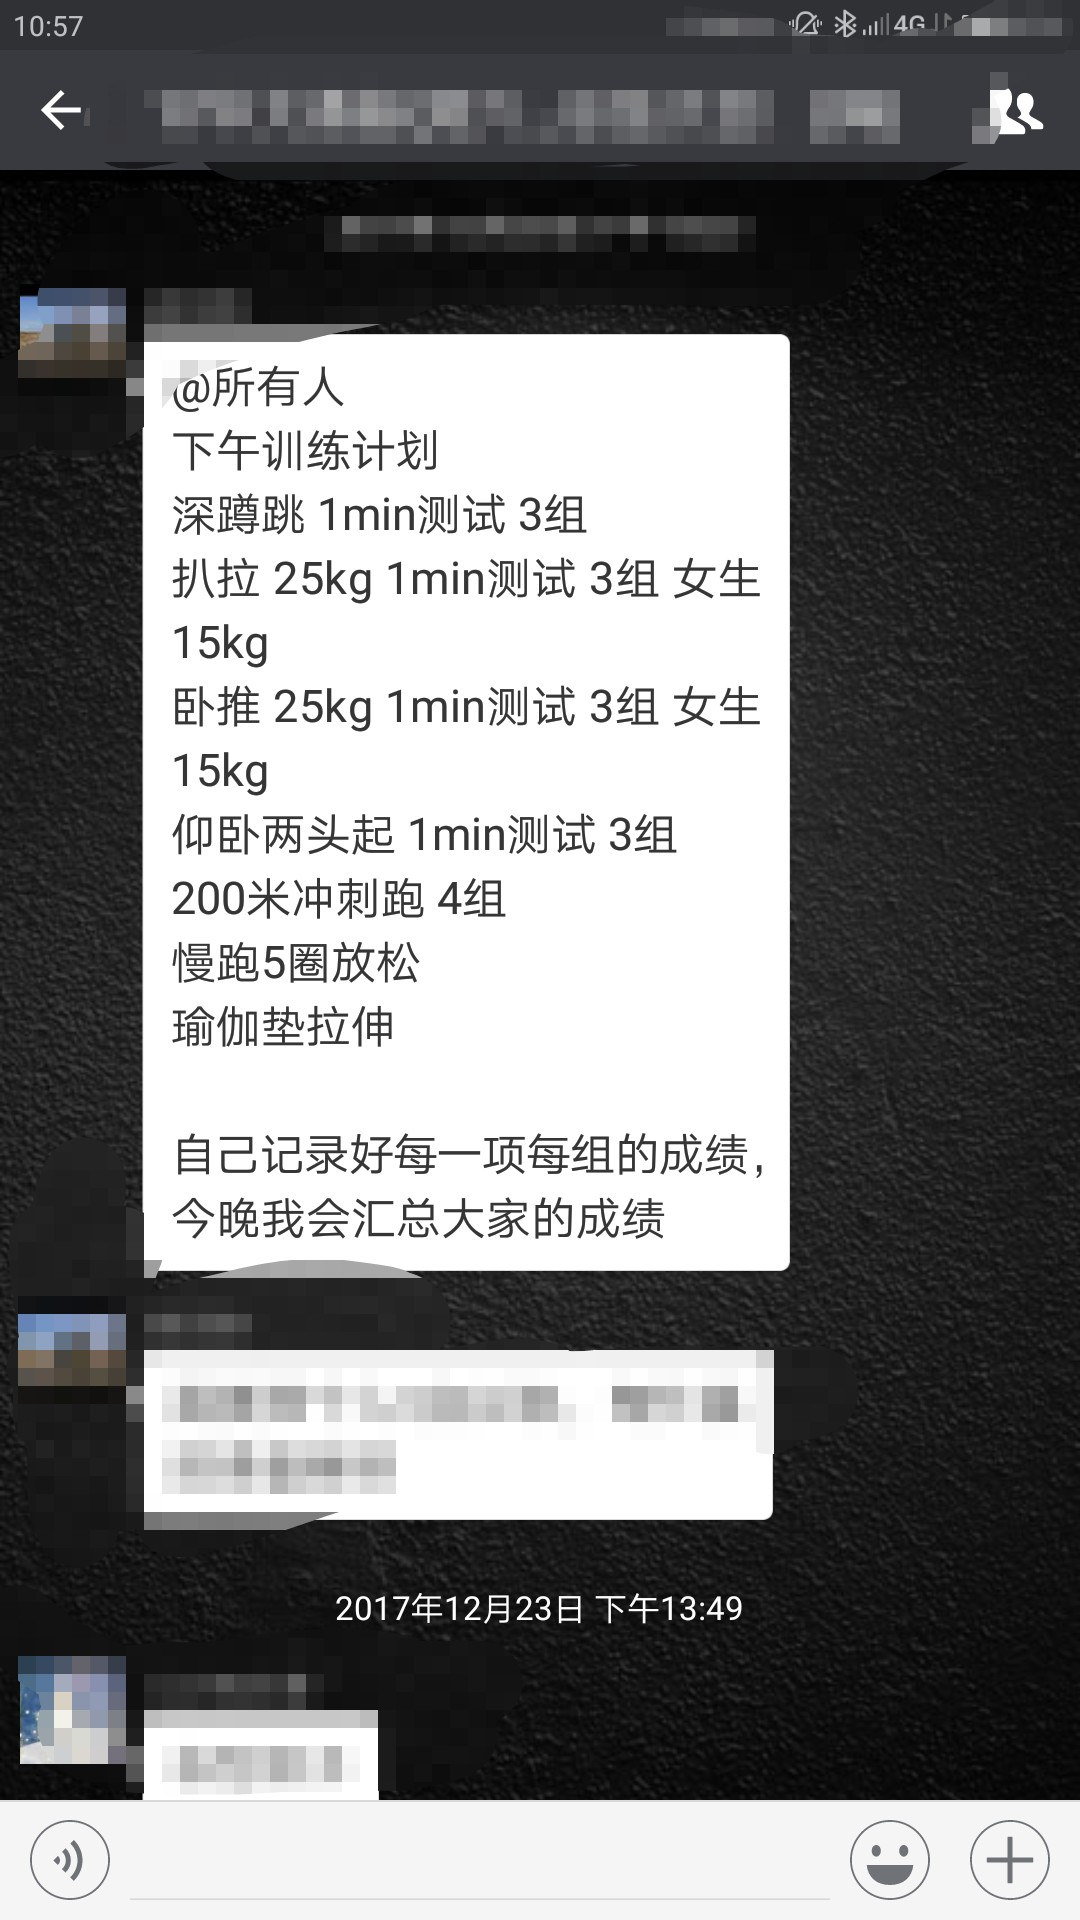
\includegraphics[scale=0.1]{pic/wechat.png}
      \column{0.5\textwidth}
      这样发布的计划和记录会在聊天记录里面分布得比较散,因此对于统计训练计划以及记
      录并进行反馈的这项工作会比较繁琐,而且数据也难免丢失,队员训练的训练反馈效果
      不会很好。
    \end{columns}
    
  }

  \only<3> {
    \begin{block}{解决方案}
    这个时候数据库应用能够简化这个工作,并给出更好的反馈。
    \end{block}
  }

  % 一个体育团队通过收集每天的训练情况来定期给队员提供积
  %   极科学的反馈,并以此能够修正训练计划,从而使训练更加高效有序。可是现实团队里面在
  %   即时通讯软件(wechat)里面发布和收集训练记录,或者说用纸来记录数据。这样的做法费
  %   时费力而且数据也不完整,即使通信软件里面有相当强大的搜索功能。但是如果每次进行数
  %   据收集都是对聊天记录进行搜索的话,数据难免丢失(数据格式不一致等原因)因此开发一
  %   个数据库应用来进行队内事务管理是相当有必要的。

  % example

  
  % One major point: State it, develop it, and repeat it.

  % Argument, evidence, and a conclusion.

  % Organize information in a highly structured fashion.

  % Clear topic sentences.
  
  % Neural machine translation is a newly emerging approach to machine translation.

  % Compress all the necessary information of a source sentence into a
  % fixed-length vector. This may make it difficult for the neural network to cope
  % with long sentences, especially those that are longer than the sentences in
  % the training corpus.

  
\end{frame}

\begin{frame}{数据库系统的设计}
  \only<1> {
    概念设计

    \begin{enumerate}
    \item
      {
        一个用户对应一个成员,有唯一的用户名作为标识符,需要密码进行登录。
      }

    \item{
        一个成员有自己的各种信息,对应唯一一个账户,有自己的训练级别,还有多条自己的
        训练记录,有多条对应自己的开支,由(ID)唯一标识。
      }

    \item{
        一个训练计划包含训练时间,训练时长,训练项目,训练指标,还有训练对应的级别,
        由(plan\_ID)唯一标识,需要和成员联系,作为计划制定者。
      }

    \item {
        一个训练记录(与训练计划对称),有训练时间,训练时长,训练项目,训练结果,由
        (record\_ID)唯一标识,需要和成员联系,作为训练者。
      }
      
    \item {船艇信息\\
        一艘艇有名字,有类型,由(ship\_ID)唯一标识。
      }

    \item {开支信息\\
        一条开支,有时间,有备注,需要和成员联系,作为支出的对象,由(fee\_ID)唯一标
        识。
      }
    \end{enumerate}    
    
  }

  \only<2> {
    逻辑设计

    \begin{itemize}
      \item user (\underline{username}, password);
      \item member (\underline{ID}, name, training\_level, info);
      \item plan (\underline{plan\_ID}, train\_at, training\_last, item(项目),
        requirements, ID);
      \item record (\underline{record\_ID}, train\_at, training\_last, item(项目),\\
        status, ID);
      \item ship (\underline{ship\_ID}, ship\_name, type);
      \item cost (\underline{fee\_ID}, time, comment, ID);
    \end{itemize}
    
    
  }

  \only<3> {
    物理设计
    限于篇幅,没法放。
  }

  % 用户信息,成员信息,训练计划信息,训练信息,艇支信息,支出信息。

  % 其中用户系统需要注意的问题是密码的储存要hash,不能用明文存储。

  % 成员系统,具体难度不大。艇支管理和支出管理不是实现的主要目的。

  % 重点则是训练计划以及训练记录信息。

  % SQL注入的防范

    
\end{frame}

\begin{frame}{设计难点}

  \only<1> {
    \begin{block}{训练记录和训练计划的设计}
      仔细看训练计划,主要有三个部分:时间,训练项目和指标。

      \begin{itemize}
      \item 一个计划可以有多个项目
        比如:深蹲,卧拉,卧推等。

      \item 其中训练项目有着各自不一样的指标。
        比如:\\
        深蹲的指标是重量,次数,组数等。\\
        跑步的指标是距离,时间等。
      \end{itemize}
    \end{block}
    
    所以指标是一个多值属性,包括\\
    \{attribute\_name,number(指标数目),comp(指标要求)\}
  }
  
  \only<2>{
    不够好的设计——将所有的指标作为属性放到计划表里面。比如这样的一个表头:

    \begin{tabular}{|l|l|l|l|l|l|l|}
      \hline
      计划索引 & 项目名字 & 距离 & 时间 & 次数 & 重量 & 需要时间\\ \hline               
      1 &       卧拉 &     NULL & NULL & 30 & 30 & NULL \\ \hline               
       1 &       平板支撑 & NULL & 2 &  NULL & NULL &          NULL \\ \hline               
       1 &       跑步 &     3000 & 14  &  NULL &        NULL &          NULL \\ \hline               

    \end{tabular}


  }

  \only<3> {
    不好的原因: 不够灵活。用书上的话来说就是冗余,不完整。

    \vspace{3em}

    冗余:很显然,表里面有很多NULL的记录。这种冗余也导致数据库的查询以及完整性约
    束的维护很难执行。

    \vspace{3em}

    不完整:假设以后要添加新的指标,比如组数,那么就要在表里增加一个新的属性。多
    出一列的NULL。而且需要判断记录是否达标的时候需要外部的应用程序做更多额外的工
    作才能判断。
    
  }
  
  \only<4>{
    解决方案

    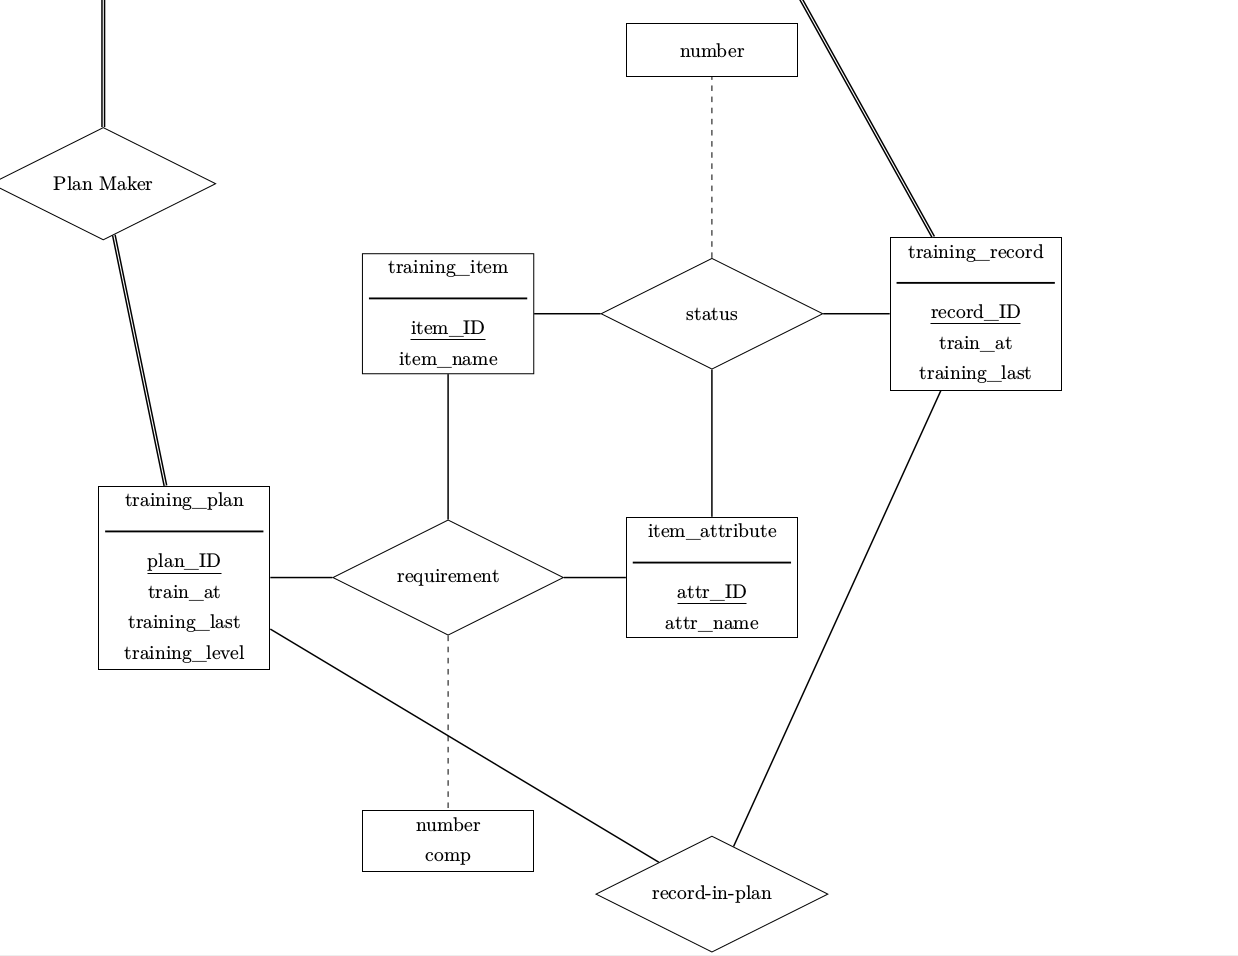
\includegraphics[scale=0.22]{pic/er-plan.png}

    % 参照完整性约束,在这个设计中,计划中的一条要求中的项目和对应的指标必须在
    % attribute\_in\_item的表中出现。
  }

  \only<5> {

    \begin{tabular}{|c|c|c|c|c|}
      \hline
      plan\_ID & item\_ID & attr\_ID & comp   & requirement  \\ \hline
      1 &       1 &       1 & larger &          30  \\ \hline
      1 &       1 &       4 & larger &          30  \\ \hline
      1 &       1 &       5 & larger &           5  \\ \hline
      1 &       2 &       3 & larger &         120  \\ \hline
      1 &       2 &       5 & larger &           2  \\ \hline
      1 &       3 &       4 & larger &          30  \\ \hline
      1 &       3 &       5 & larger &           2  \\ \hline
      \end{tabular}

    好处:
    \begin{enumerate}
    \item 灵活性,把指标作为一个实体。
    \item 减少冗余性。
    \item 有更好的表达性。
    \end{enumerate}
  }
    
\end{frame}
  
\begin{frame}{展示}
\url{http://120.79.66.205:5000}
\end{frame}

\end{document}
%%% Local Variables:
%%% TeX-engine: xetex
%%% end: